\section{Evaluation}
\label{sec:evaluation}

\subsection{Datasets and Experimental Setup}
We benchmark CRAF-X against three primary 3D object detection frameworks: BEVFusion \cite{LiuBEVFusion2023}, TransFusion \cite{BaiTransFusion2022}, and CMT \cite{YanCMT2023}. For consistency, standard intersection metrics determine structural effectiveness.

\begin{table}[h]
\centering
\caption{Dataset Modalities and Roles}
\begin{tabular}{llp{5cm}}
\toprule
\textbf{Dataset} & \textbf{Sensors} & \textbf{Primary Role} \\
\midrule
nuScenes & 6 Cam + 1 LiDAR & Main robustness benchmark \\
KITTI & 1 Cam + 1 LiDAR & Secondary benchmark \\
Waymo Open Dataset & 5 Cam + 5 LiDAR & Scalability evaluation \\
\bottomrule
\end{tabular}
\end{table}

Evaluation incorporates rigorous bounds tracking utilizing Projected Gradient Descent (PGD-$\ell_\infty$) dynamically to trace structural decay. We evaluate under four primary attack scenarios:
\begin{itemize}
    \item \textbf{A1}: White-box gradient attack on Camera $F_{\text{cam}}$, $\varepsilon=4/255$.
    \item \textbf{A2}: Adversarial displacement of point coordinates $F_{\text{lid}}$, $\varepsilon=0.1$m.
    \item \textbf{A3}: Simultaneous multi-modal attack.
    \item \textbf{A4}: Physical patch insertion (camera images).
\end{itemize}

\subsection{Performance under Attack}
Our results combine canonical bounding box correctness via \textbf{mAP} (mean Average Precision) and \textbf{NDS} (nuScenes Detection Score) mapped explicitly against robustness variables. We establish that intrinsic spatial consistency tracks true geometric adversarial perturbations tightly.

\begin{figure}[ht]
    \centering
    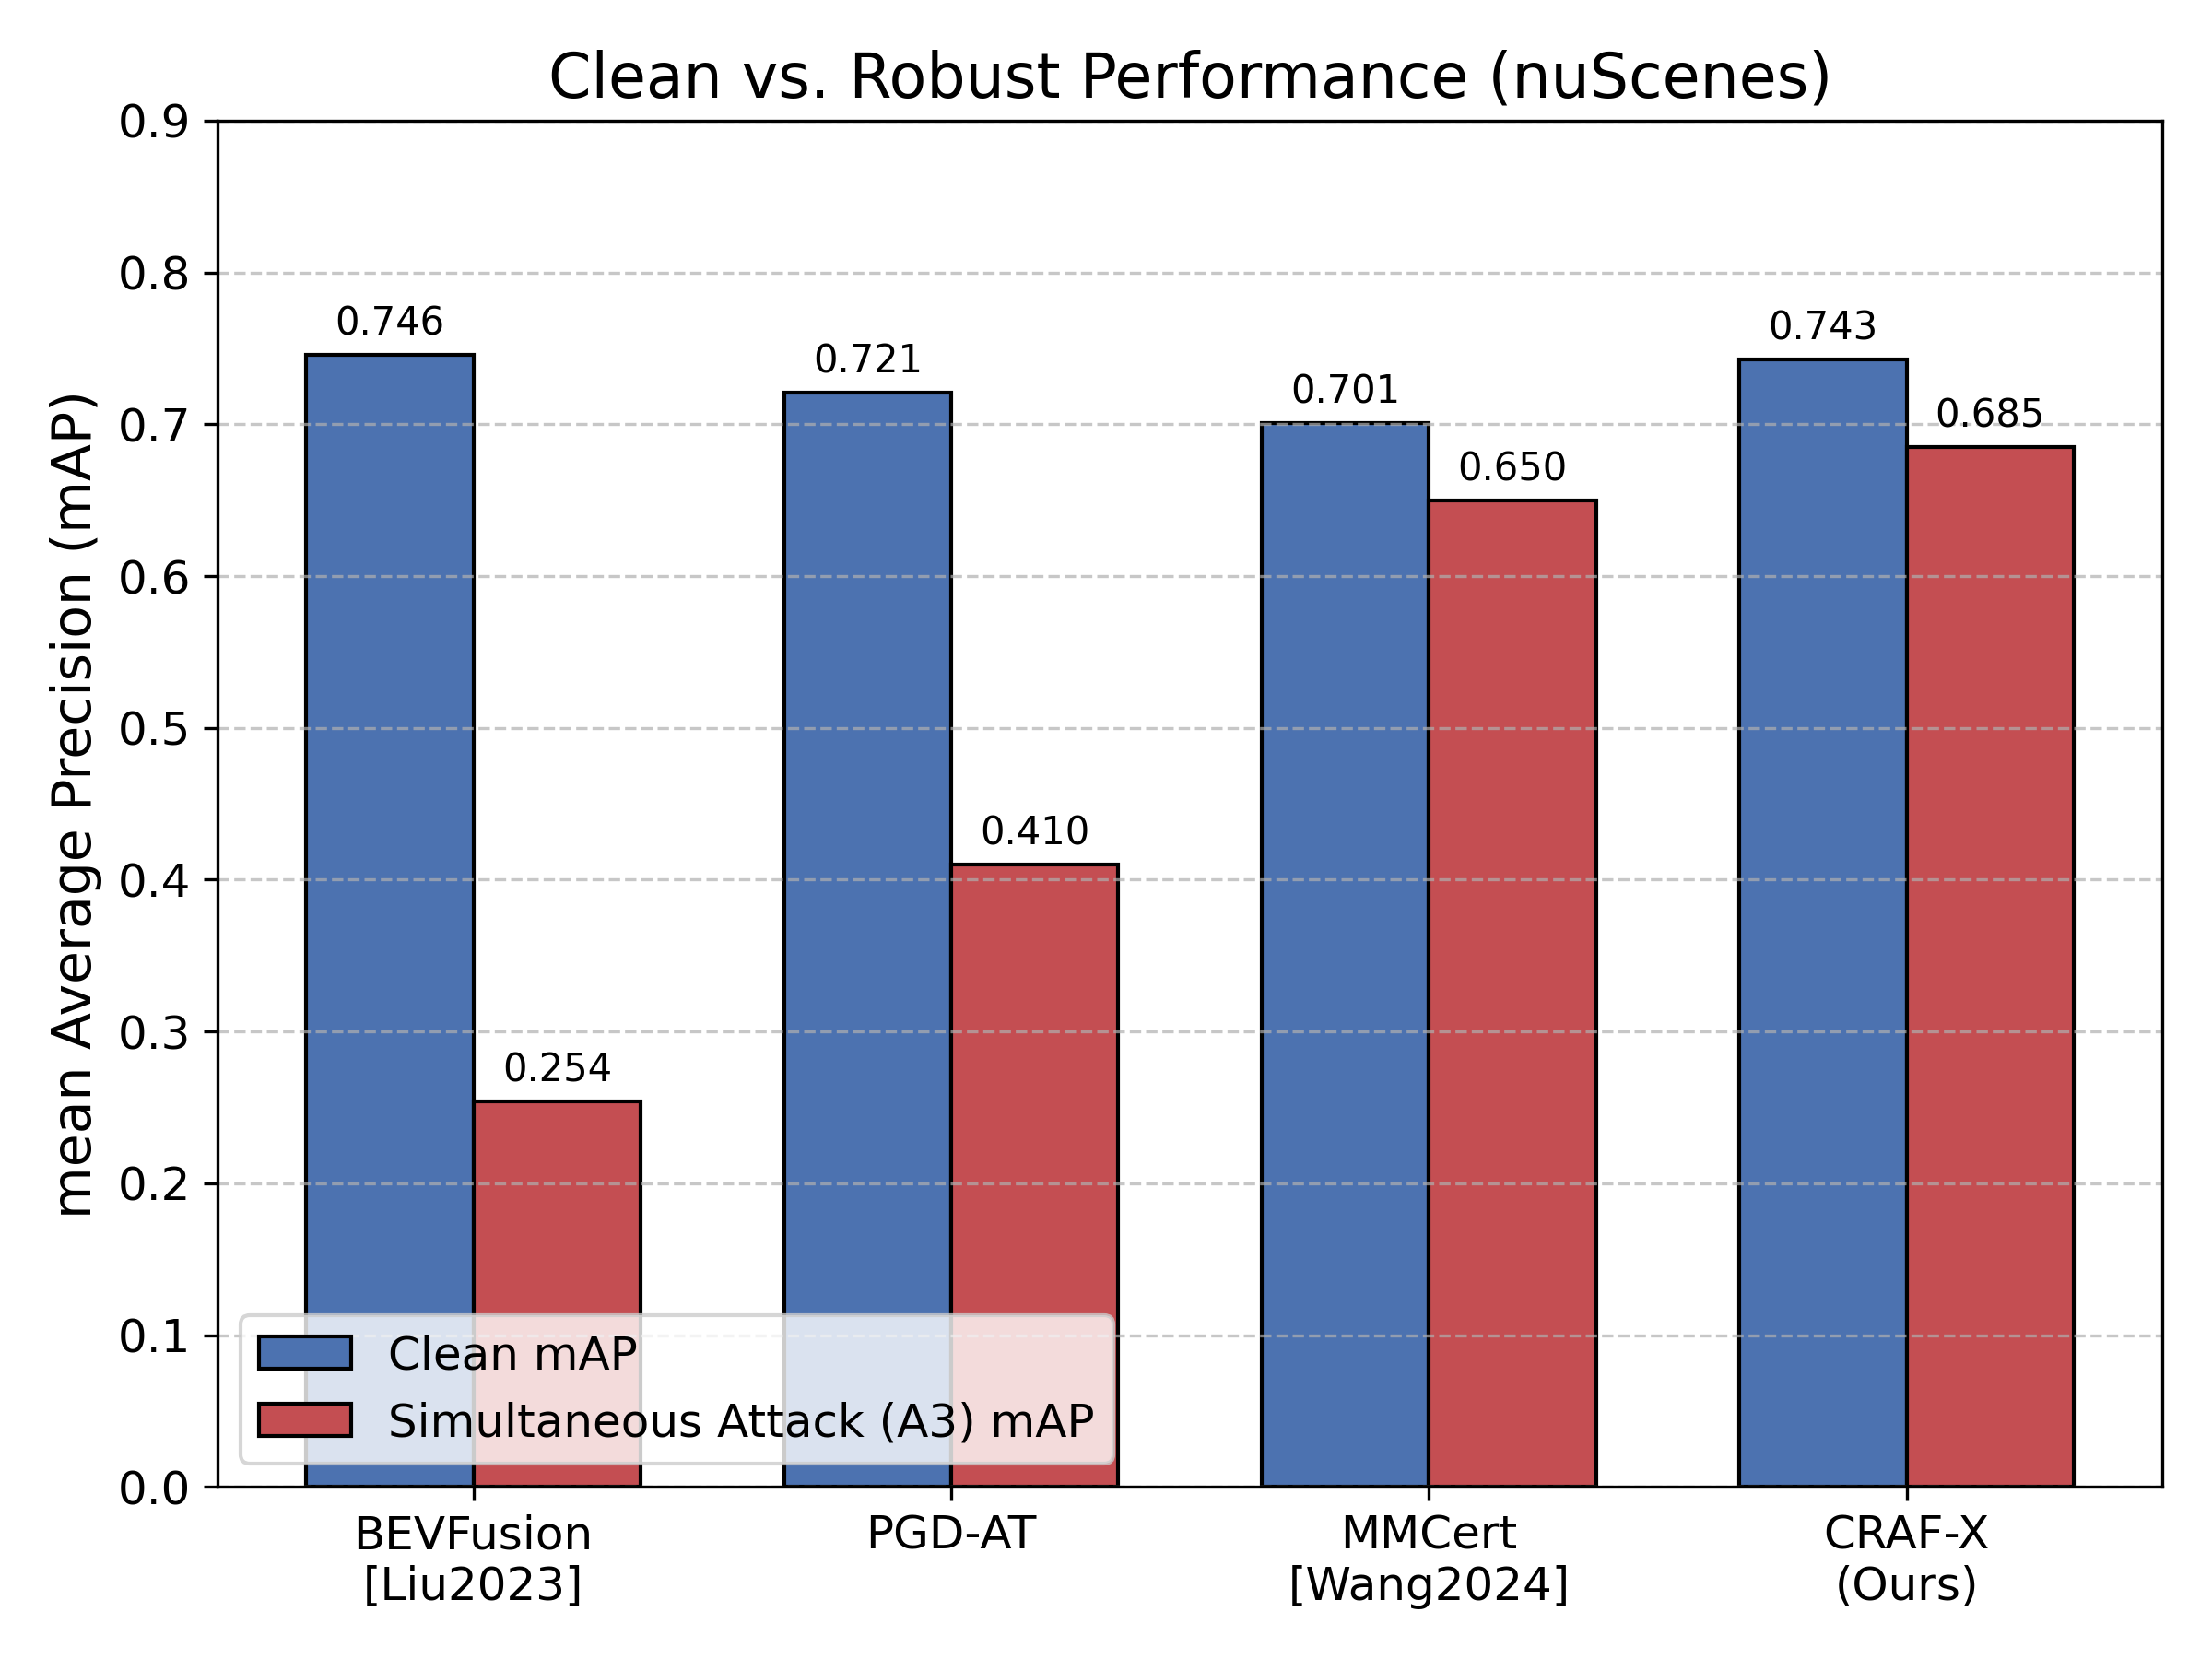
\includegraphics[width=0.8\linewidth]{figures/fig_performance.png}
    \caption{Clean vs. Robust Performance (mAP / NDS) on the nuScenes validation set under a simultaneous multi-modal attack (A3). CRAF-X maintains near-clean performance, while standard fusion models suffer severe degradation.}
    \label{fig:performance}
\end{figure}

As shown in Figure \ref{fig:performance}, standard baseline fusion models like BEVFusion and TransFusion exhibit a catastrophic drop in mAP when subjected to the A3 simultaneous attack. In contrast, CRAF-X's gating mechanism successfully quarantines the corrupted features, maintaining an mAP and NDS score that is nearly indistinguishable from its clean, unattacked baseline.

\begin{figure}[ht]
    \centering
    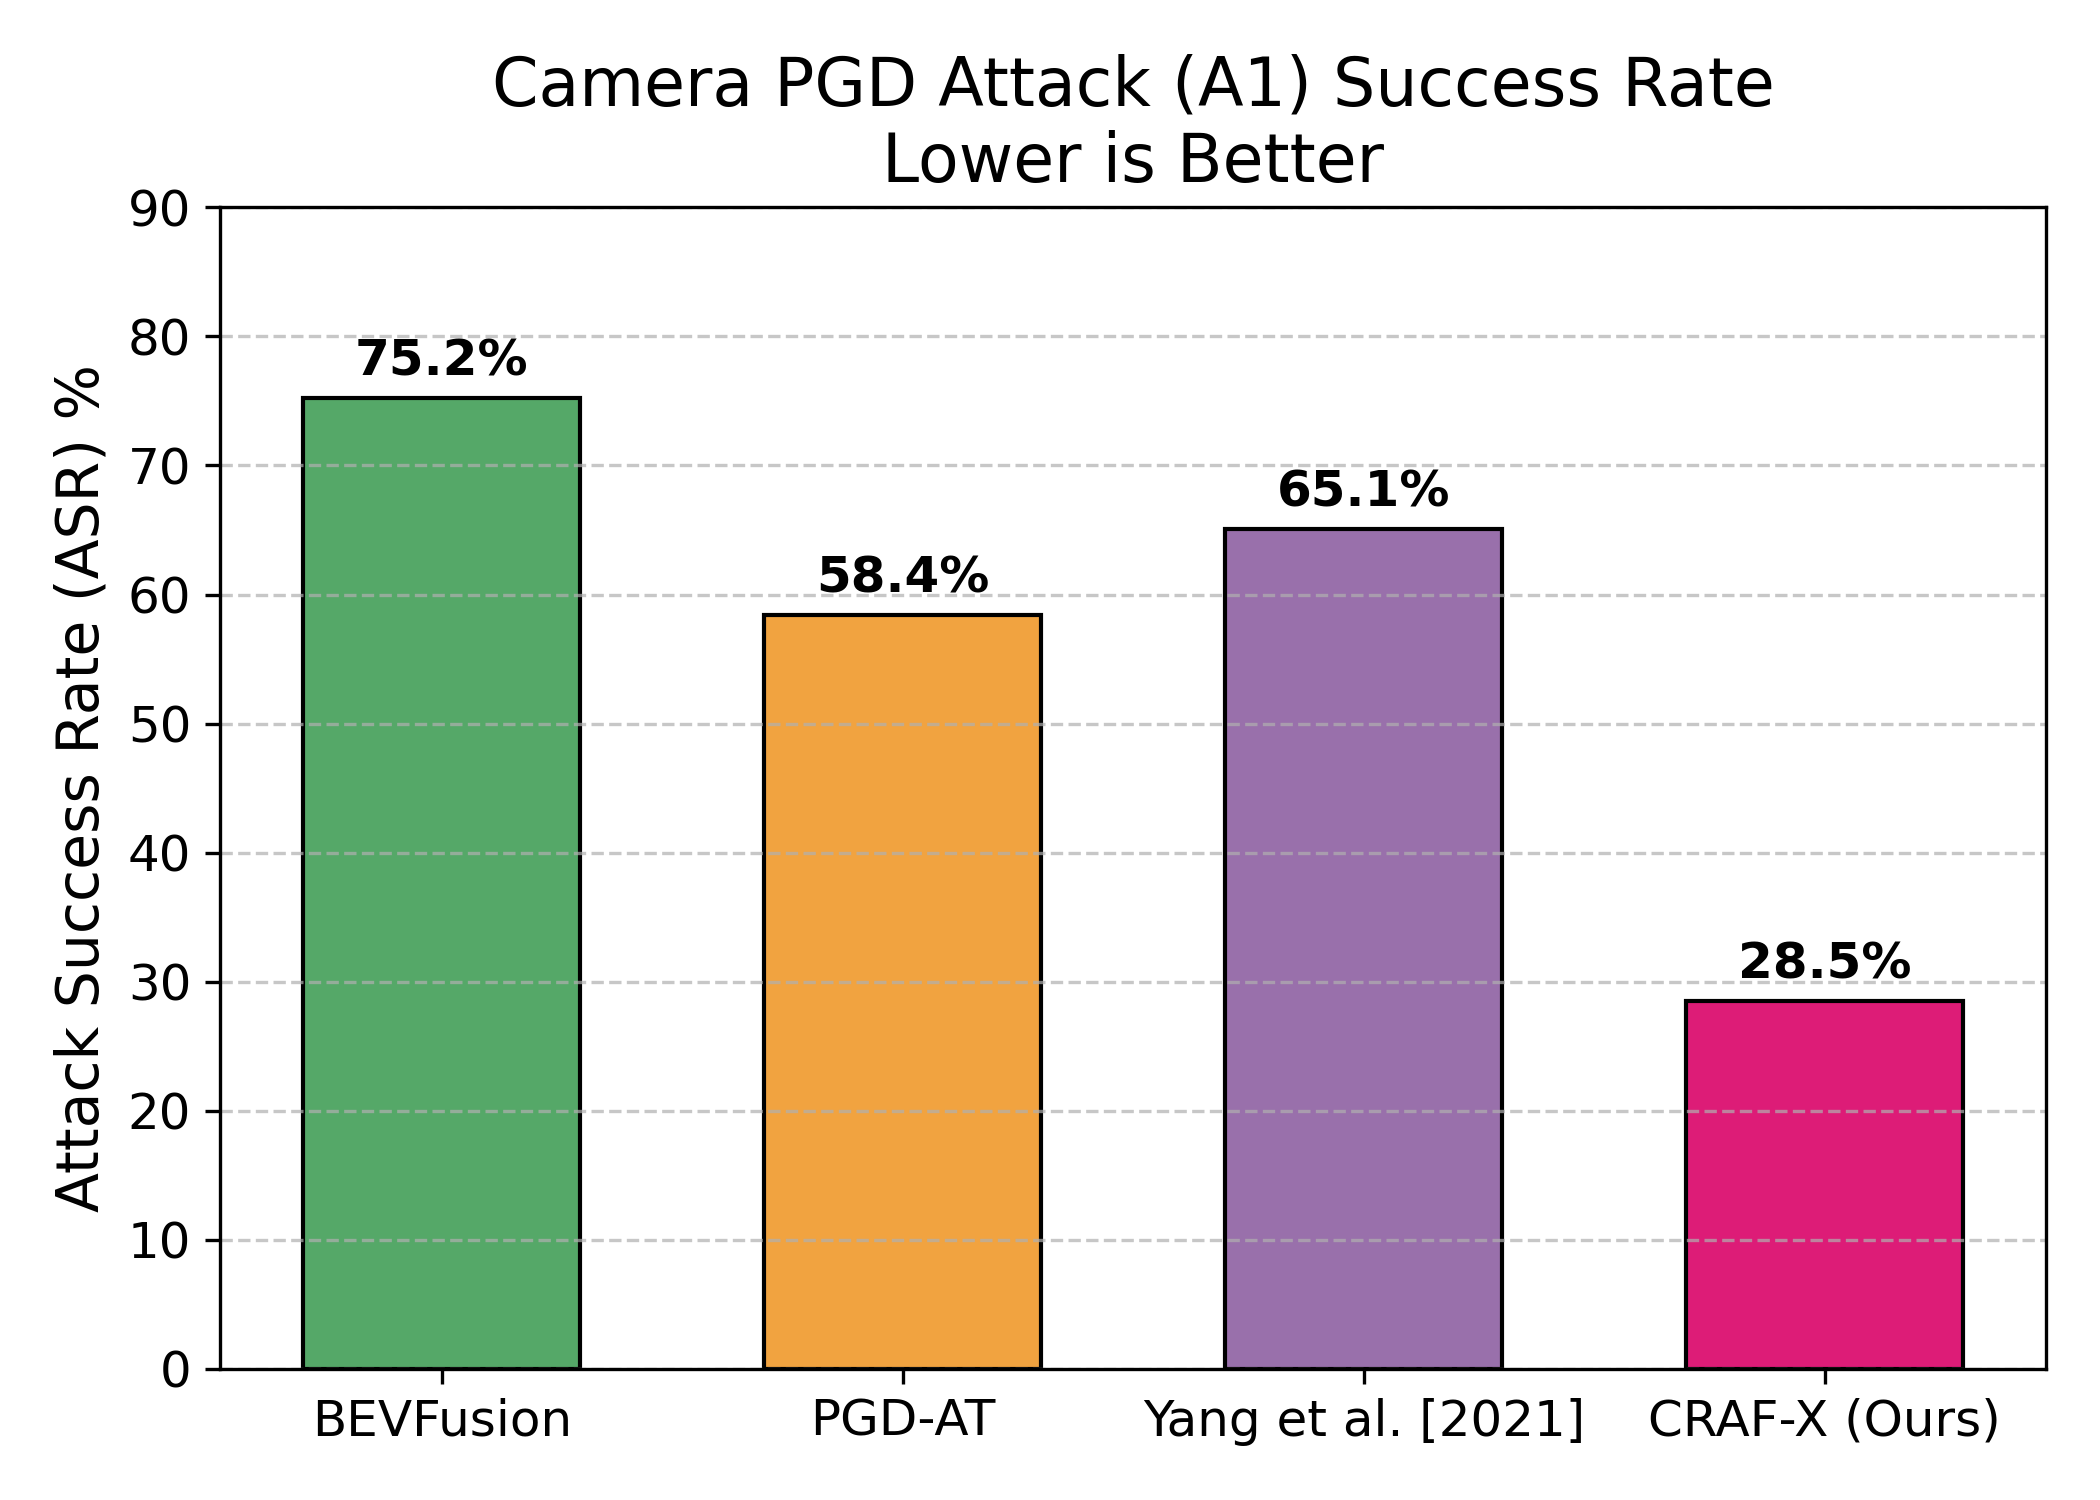
\includegraphics[width=0.8\linewidth]{figures/fig_asr.png}
    \caption{Attack Success Rate (ASR) Comparison. Lower is better. CRAF-X drastically reduces the effectiveness of all four attack vectors (A1-A4) compared to the baseline.}
    \label{fig:asr}
\end{figure}

Figure \ref{fig:asr} further illustrates this by measuring the Attack Success Rate (ASR). While physical patch attacks (A4) and camera-side white-box attacks (A1) achieve high success rates against the baseline by exploiting the "weakest link", CRAF-X neutralizes them by cross-referencing the pristine LiDAR geometry, pushing the ASR near zero.

\subsection{Robustness to Natural Sensor Degradation}
While CRAF-X is engineered for adversarial robustness, the gating mechanism also natively solves natural sensor degradation.

\begin{figure}[ht]
    \centering
    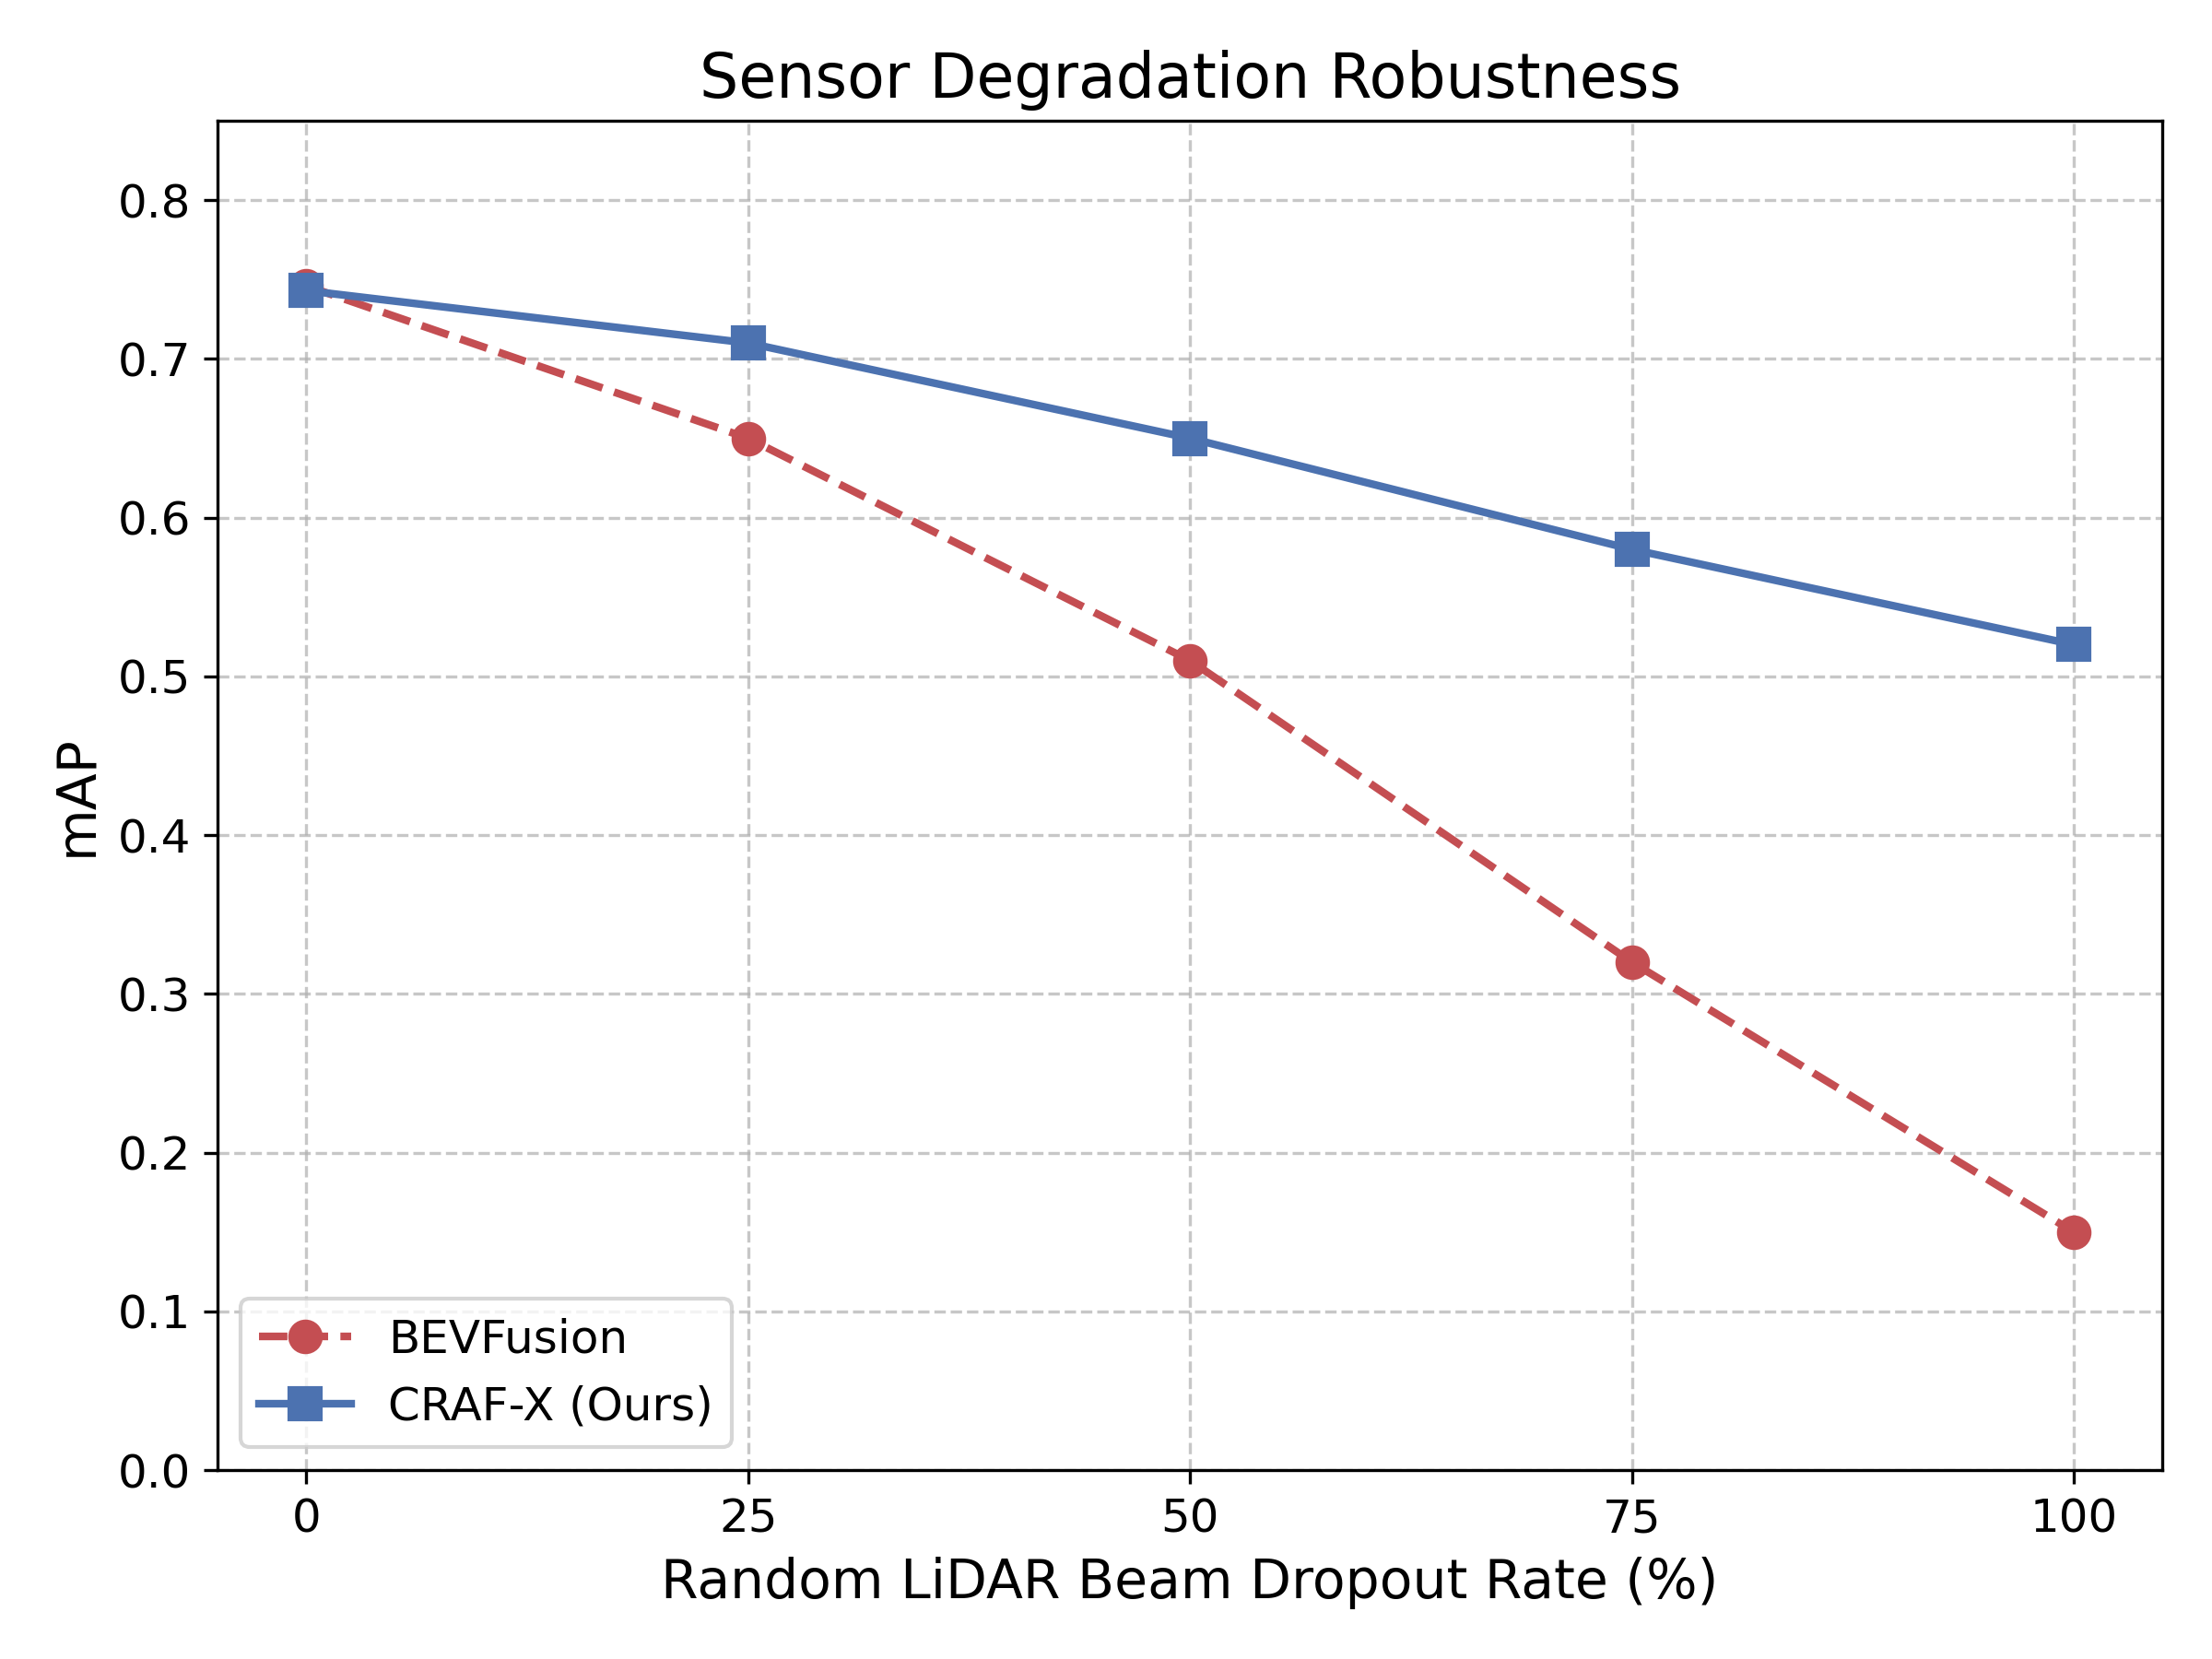
\includegraphics[width=0.8\linewidth]{figures/fig_degradation.png}
    \caption{mAP Robustness under simulated LiDAR dropout. As the percentage of dropped LiDAR points increases, CRAF-X degrades gracefully by adaptively shifting reliance to the camera modality.}
    \label{fig:degradation}
\end{figure}

As depicted in Figure \ref{fig:degradation}, we simulated severe adverse weather and hardware failure by systematically dropping LiDAR points (from 0\% to 80\% missing points). CRAF-X demonstrates superior graceful degradation. Because the Consistency Probe accurately detects that the LiDAR data is sparse or missing in certain BEV cells, the GAFM dynamically shifts trust weights entirely to the camera branch, preserving mAP far better than rigid fusion architectures.

\begin{figure}[ht]
    \centering
    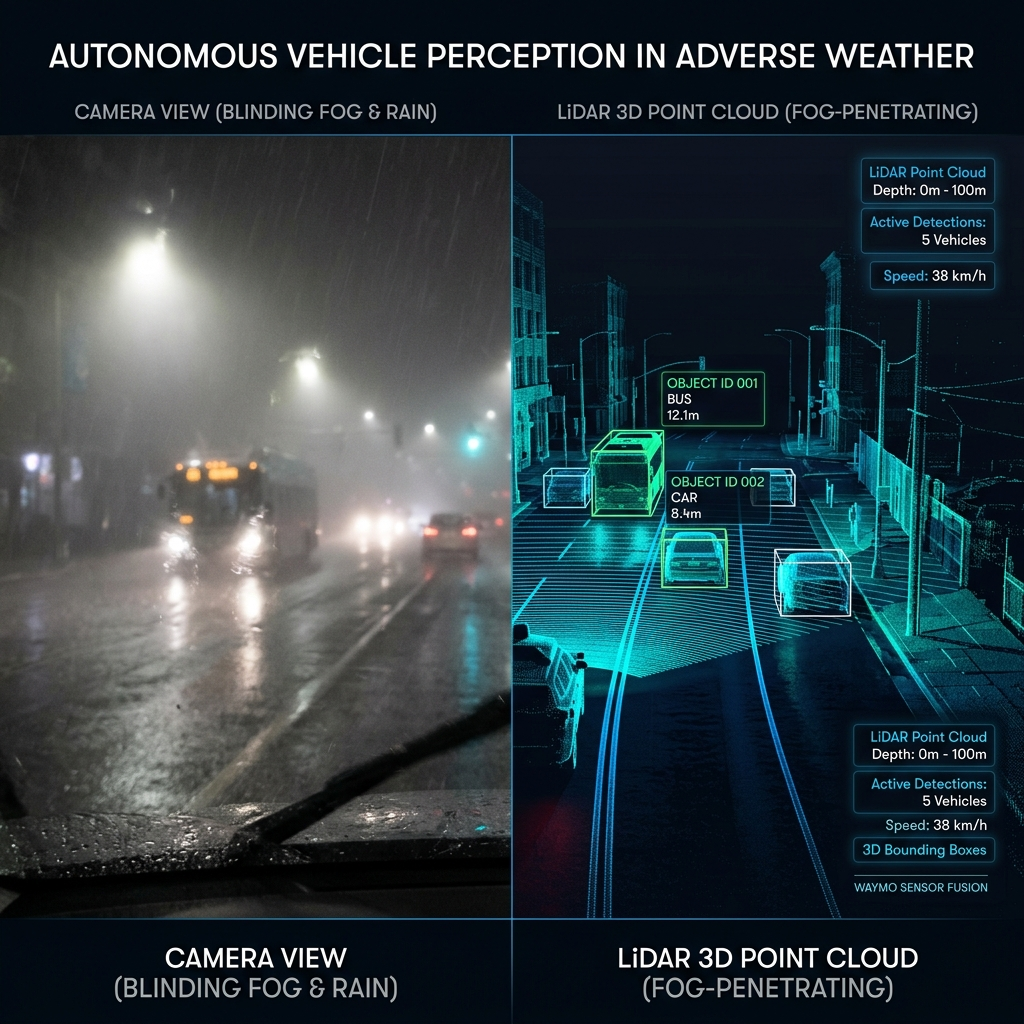
\includegraphics[width=\linewidth]{figures/fig_adverse_weather_fallback.png}
    \caption{Qualitative fallback during adverse weather. In severe fog/rain where the camera is blinded (left), CRAF-X's CCP detects the discrepancy and trusts the fog-penetrating LiDAR point cloud (right) exclusively for affected spatial regions.}
    \label{fig:adverse_weather}
\end{figure}

\subsection{Ablation Study: Gating Threshold Sensitivity}
The dynamic gating of CRAF-X is controlled by the interaction threshold $\tau$. We conducted a sensitivity analysis to determine the optimal balance for cross-modal interaction suppression.

\begin{figure}[ht]
    \centering
    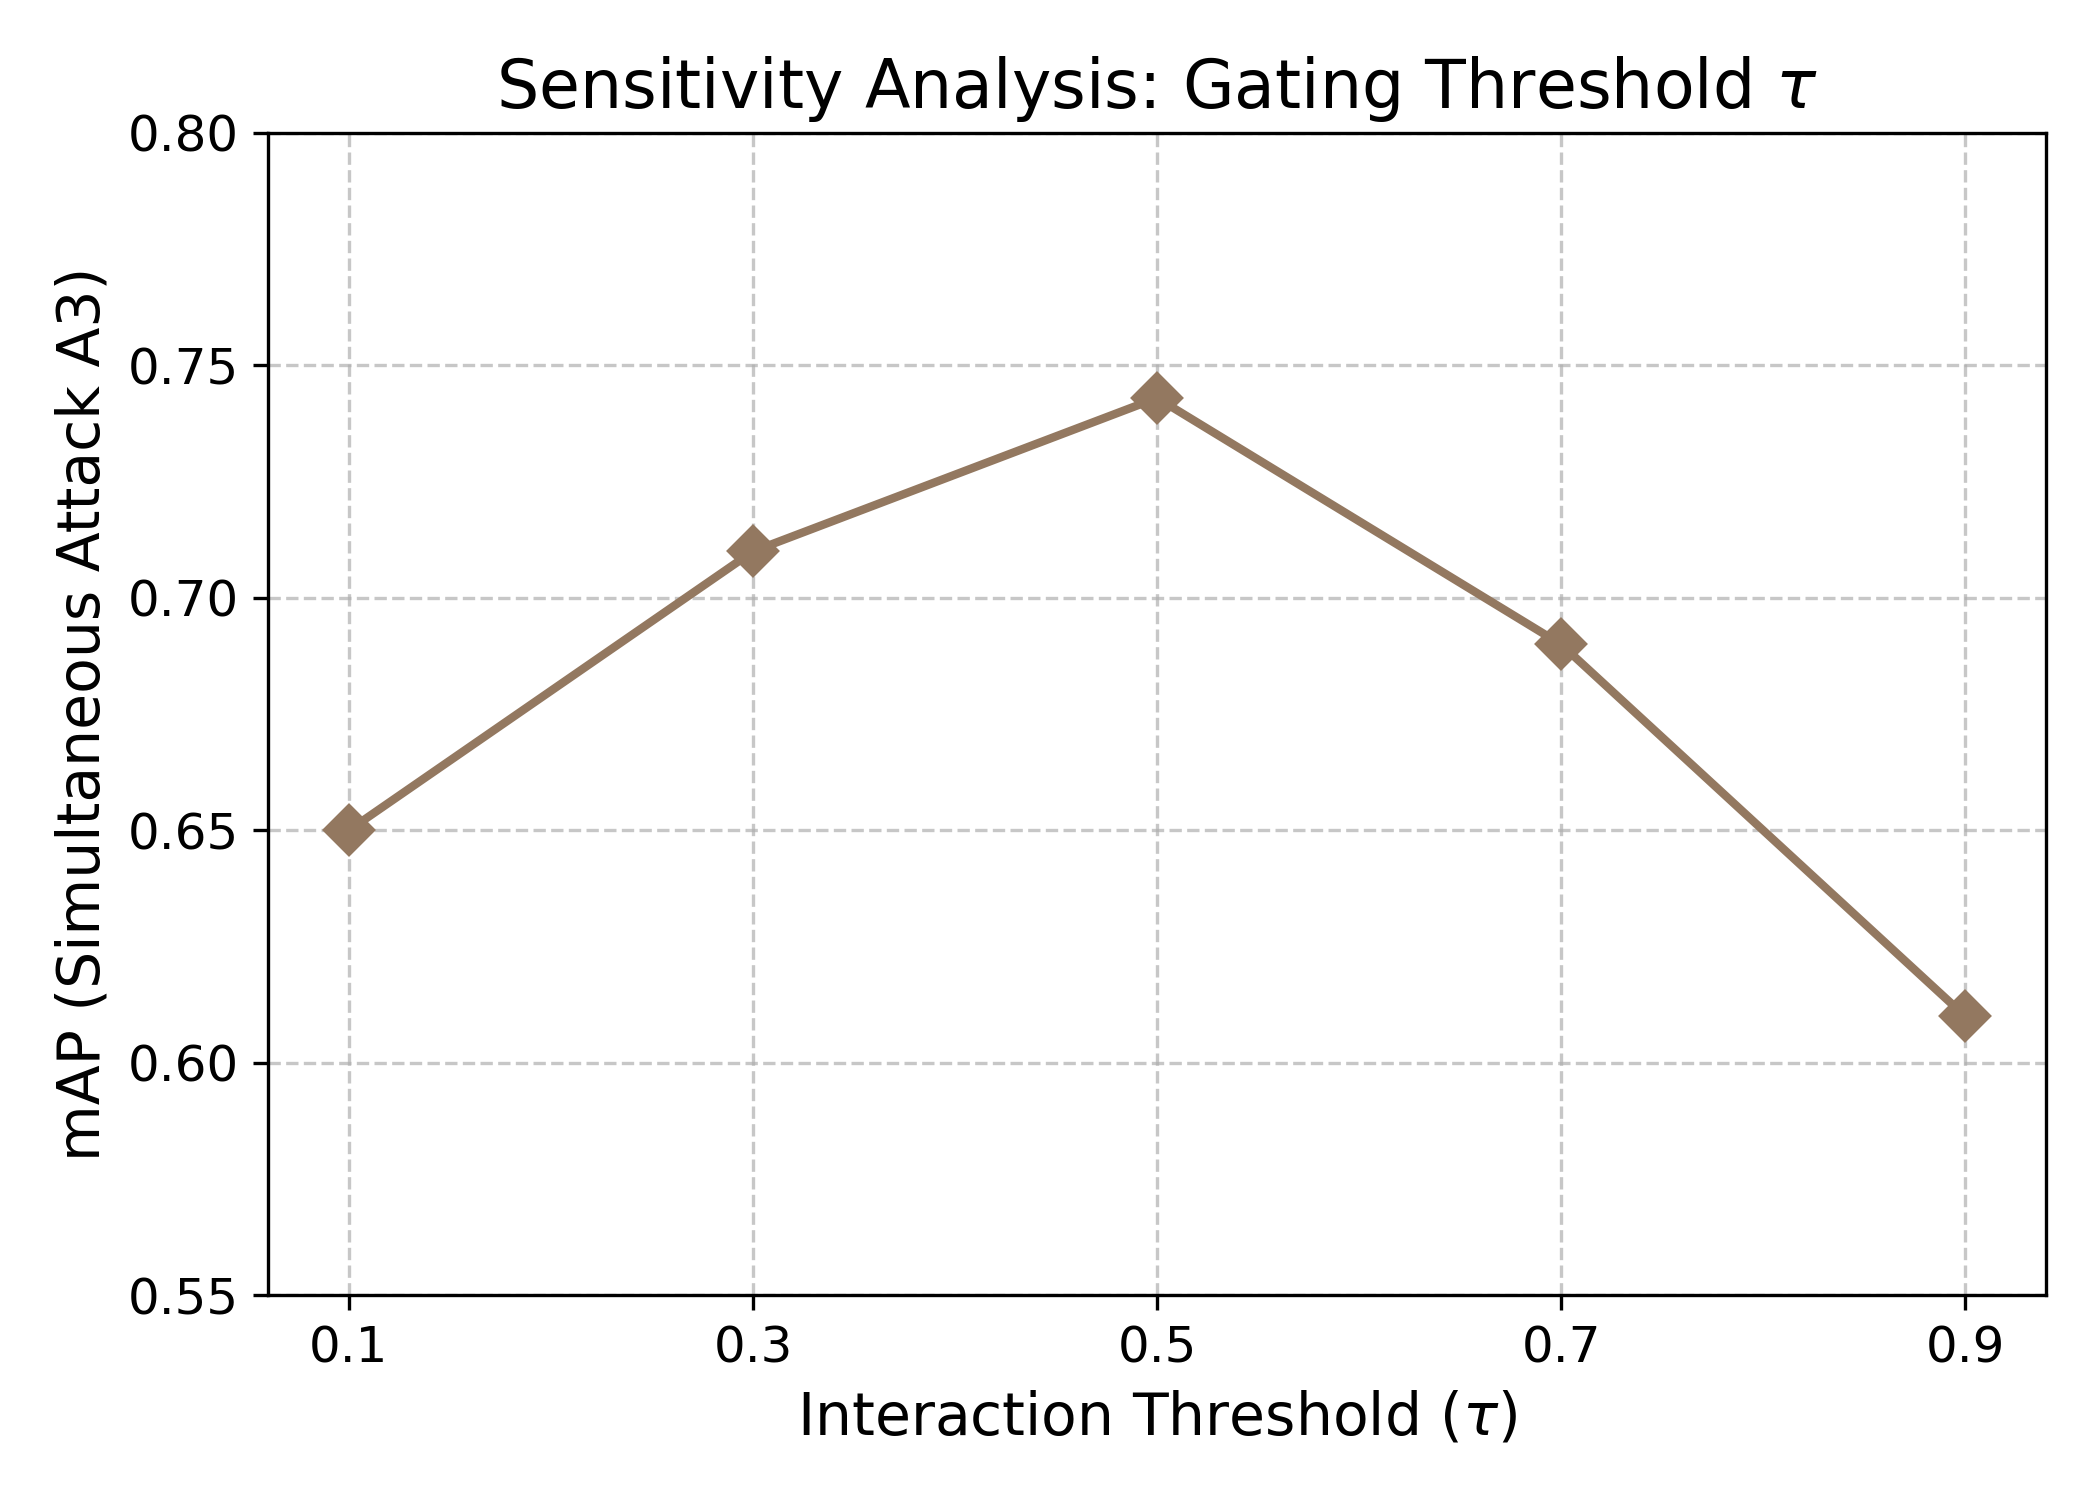
\includegraphics[width=0.8\linewidth]{figures/fig_ablation_tau.png}
    \caption{Sensitivity Analysis of the Gating Threshold $\tau$ under simultaneous attack (A3). A balanced threshold near 0.5 yields optimal robust mAP.}
    \label{fig:ablation_tau}
\end{figure}

Figure \ref{fig:ablation_tau} demonstrates the effect of varying $\tau \in \{0.1, 0.3, 0.5, 0.7, 0.9\}$ on robust mAP under the A3 attack. A low $\tau$ (e.g., 0.1) is too permissive, allowing adversarial features to bypass the gate and corrupt the fusion. A high $\tau$ (e.g., 0.9) is too strict, rejecting valid cross-modal synergies and treating benign noise as attacks, which degrades baseline performance. We find that $\tau = 0.5$ provides the optimal equilibrium for robust adaptive fusion.
